\normalfont\normalsize
\chapter{Software Implementation}

The solution is divided into different modules that run independently  but communicate with each other to achieve the main goal. The separation of software modules allows for future features to be added easily.

The main modules are installed in the AR Parrot Drone and the Android FreeFlight 2.0 application.

The SparrowDongle gateway is always in a listen-for-data state and dumps any data received on the serial. When it receives the data, it sends back an ACK message back to let the SparrowV3.2 node to know that it can begin sending the entire stored data to the mobile gateway.

The SparrowV3.2 node is sending periodically a small data packet to check if a gateway is available. It stores the data accumulated over the period when no reply is given to it. When it receives the ACK message from a mobile gateway it starts sending the stored data to the gateway. The data sent can vary, from sensor readings to debugging information in order to check the state of the Wireless Sensor Network.

The data gathered by the gateway is saved into different files in the AR Parrot Drone's internal memory. The files also contains information such as the node identification tag and time of the transfer. The data can be accessed at any time by any device connected to the drone's wireless network port 4242 via FTP.

The drone also processes some of the collected data to provide realtime HUD information, such as signal strength, last connection time and number of discovered nodes. This information is sent to the controlling device through a socket connection.

The controlling device, pc or android, will gather the information and display them to the user.

\clearpage

\begin{figure}[ht]
\begin{center}
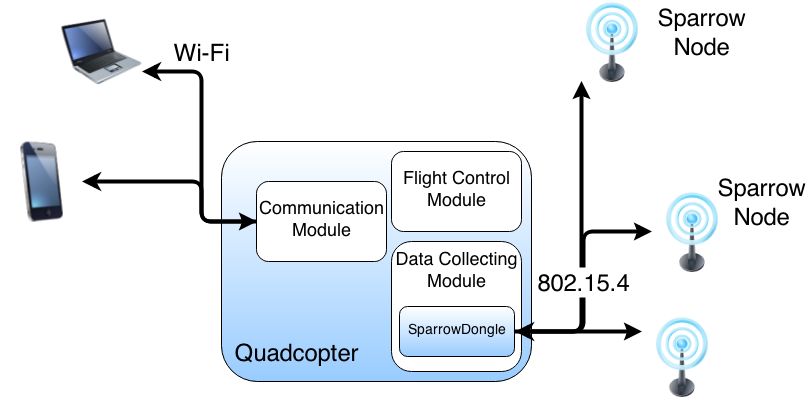
\includegraphics[width=0.9\textwidth]{implementation/organigrama.png}
\end{center}
\caption{\small \itshape{Modules and connections between them and devices}}
\end{figure}

\section{The Debug Module}

% Trebuie descris mai clar de ce e nevoie de Debug Module și ce face
When performing modification to the existing code, a debug enabling option whould speed up the process. The moudle whould allow for displaying controll message to the user console even when the process is running in background.If the messages would be activated all the time, they would slow down the execution speed of the process.

In order to see those messages, the debug option must be activated and then this simple command whill show them:

\lstset{numbers=none, mathescape=true, nolol=false,caption=Simple display message command,label=lst:task}
\begin{lstlisting}
p=$(pidof read) \&\& strace -p $p
\end{lstlisting}

Enabling the debug is just a matter of setting  a define from 0 to 1, recompile and upload the code to the drone to see the messages.

\lstset{numbers=none, mathescape=true, nolol=false,caption=Data Collection use of mutex,label=lst:task}
\begin{lstlisting}
/* activates/deactivates printf debug information*/
#define DEBUG_ON 0
/* delay yime in microseconds*/
#define DELAY_US 100000
#define DEBUG_PRINT(a...) { if(DEBUG_ON) printf(a); }
\end{lstlisting}

Also, in certain parts of the modules, a wait action is needed in order to wait for an action to be executed. The value can be changed to any level, but you must be carefull in doing this. A small delay will send data more often but it could use alot of processing power, while a big delay could be to slow for the data to be usable. Now the delay is set at 100 ms, for a 10 times per second data update.



\section{The Data Collecting Module}

The module saves the collected data into the drone's internal memory and pases the data on to the communication module, which will display on the controller interface certain data: number of nodes currently connected to the Dongle, de signal strength, if the Dongle is connected etc.

This module, besides the main purpose and similar to the other modules, has some extra features that are design to make the solution more user friendly and easier to improve in the feature.

\subsection{Modules intercommunication}

The memory area in which the information sent to the user is saved is shared between this module and the communication module. The interaction method between these two modules belongs to the consumer-producer archetype, where the Data Collecting Module can be associated with the producer side and the Communication Module with the consumer side.

A sensible issue with this approach regards possible deadlocks. This is prevented with the use of a mutex construct that allows only one thread at a time to modify the data.

\lstset{numbers=none, mathescape=true, nolol=false,caption=Data Collection use of mutex,label=lst:task}
\begin{lstlisting}
pthread_mutex_lock(&data_lock);
add_node_data(get_current_timestamp(),read_data + 7);
pthread_mutex_unlock(&data_lock);
\end{lstlisting}

The mutex is used similarly in the Communication Module when it consumes the information.


\subsection{Fault tolerance}

Because the Dongle is connected to an USB port on a machine that has a lot of vibrations, it might desconnect / reconnect for a very short period of time, so this module has been designed  with multiple USB disconnects and reconnects without the need to reset the Drone. This infomation is vital, because you can check if the Dongle is still connected to the dron without the need to inspect it visualy or to connect to a debug terminal.

\section{The Communication Module}

All of the information gathered by the Data Collecting Module would be useless if it cannot be accessed easily.

This module, as the name suggests, handles the communication of this this crucial information back to the user.

Being a different module, with different attributions than the Data Collecting Module, it has an entire Linux process dedicated to it for 3 important reasons:
\begin{enumerate}

\item The approach of having a process per module allows the modules to run independently of each other;
\item The Data Collecting Module can collect the data from the Dongle as soon as this is available;
\item If the Communication Module stops working, the Data Collecting Module can keep collecting data, so complete failure of the system is avoided;
\item System processes can be restarted in case of failure.

\end{enumerate}

\subsection{Socket with connection reset}

The communication is done through socket connections listening on port 8888. The server running on the drone accepts only one connection at a time.

If a connected client decides to disconnect before or while a write operation is in progress, a SIGPIPE error signal will be thrown, stopping all the modules. This is prevented by ignoring the signal, forcing the write action to return a EPIPE, and exiting gracefully.

The main process will use the callback \texttt{ accept\_socket\_connection} to reestablish a new connection. Once a connection is established, it will send information once every DELAY\_US microseconds. The program was configured and tested with a 100 ms wait period that leads to a ten times per second information update.

This delay is required because:
\begin{itemize}

\item If data is send too often, the socket might be flooded and stop sending the data. %?
\item If there was no delay, it would occupy too much processor time both for the drone and the controlling device.

\end{itemize}

\subsection{JSON Encoding of Data} \cite{json}

% Mai pe larg
JSON is an open-standard that uses text to encode data and it is an alternative to XML.

JSON is best suitable for this application as a data encode format becuase it is data oriented, unlike XML which is document oriented. 

Also it is very easy to encode, the result is smaller than the XML alternative and all devices can decode it. 

The informations encoded are
\begin{itemize}

\item Dongle connection status
\item An array containing node data
\begin{itemize}

	\item Node unique ID
	\item Last connection time of the node to Dongle
	\item The power of the received signal

	\end{itemize}
\end{itemize}
 


\section{Android application modules}

\begin{figure}[ht]
\begin{center}
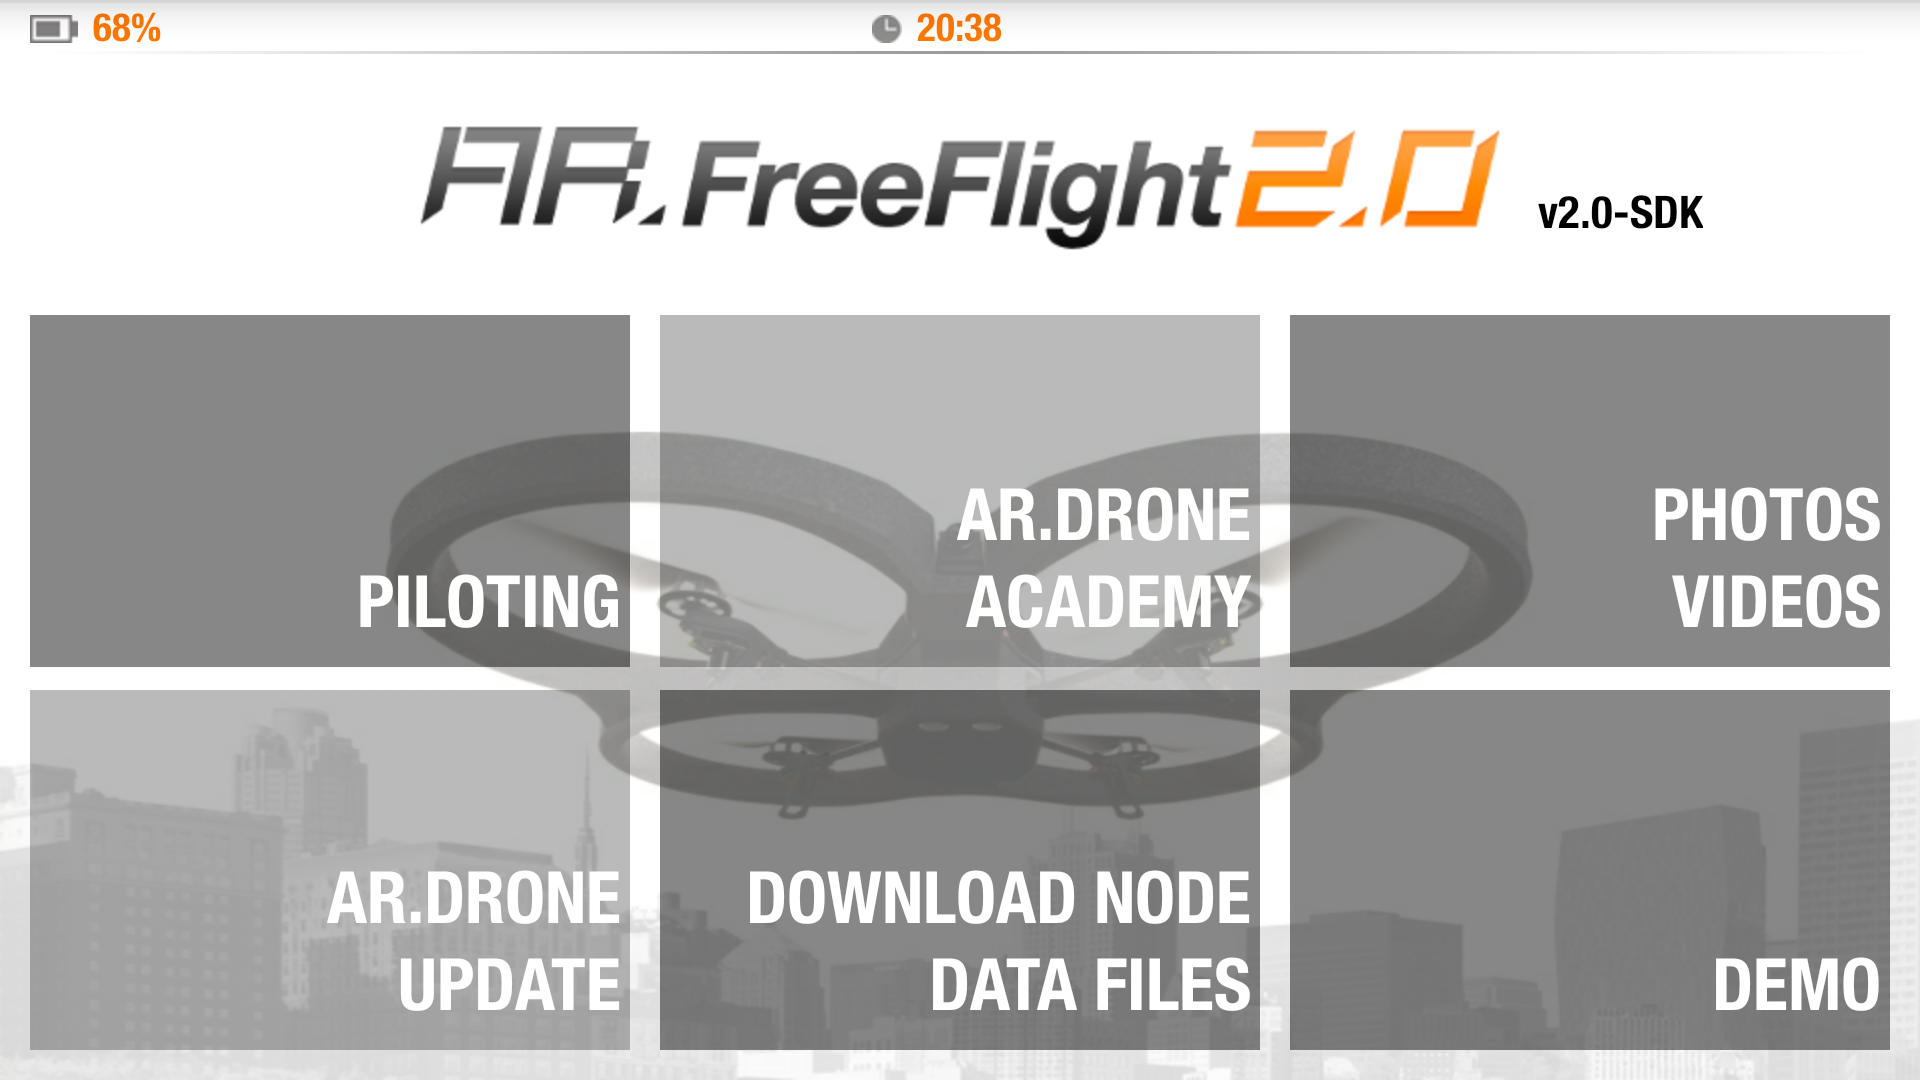
\includegraphics[width=0.9\textwidth]{implementation/android_app.png}
\end{center}
\caption{\small \itshape{ARFreeflight modified application}}
\end{figure}

Being an open-source platform we have modified the AR Freeflight 2.0 Android application to communication with our new modules added to the drone.

% cum adică fairly
%% am modificat putin
Android fairly imposes the use of the background process class AsynkTask when you have to use communication protocols like http, ftp, sockets because this prevents the UI process from being stuck in communication and not responding to user actions.

The class offers 5 very important methods that can be overwritten, 3 running on the main UI process, that prepare data before and after execution, publish the progress or simply cancel at any step, and 1 running on the actual background process.


\subsection{Display information module}

\begin{figure}[ht]
\begin{center}
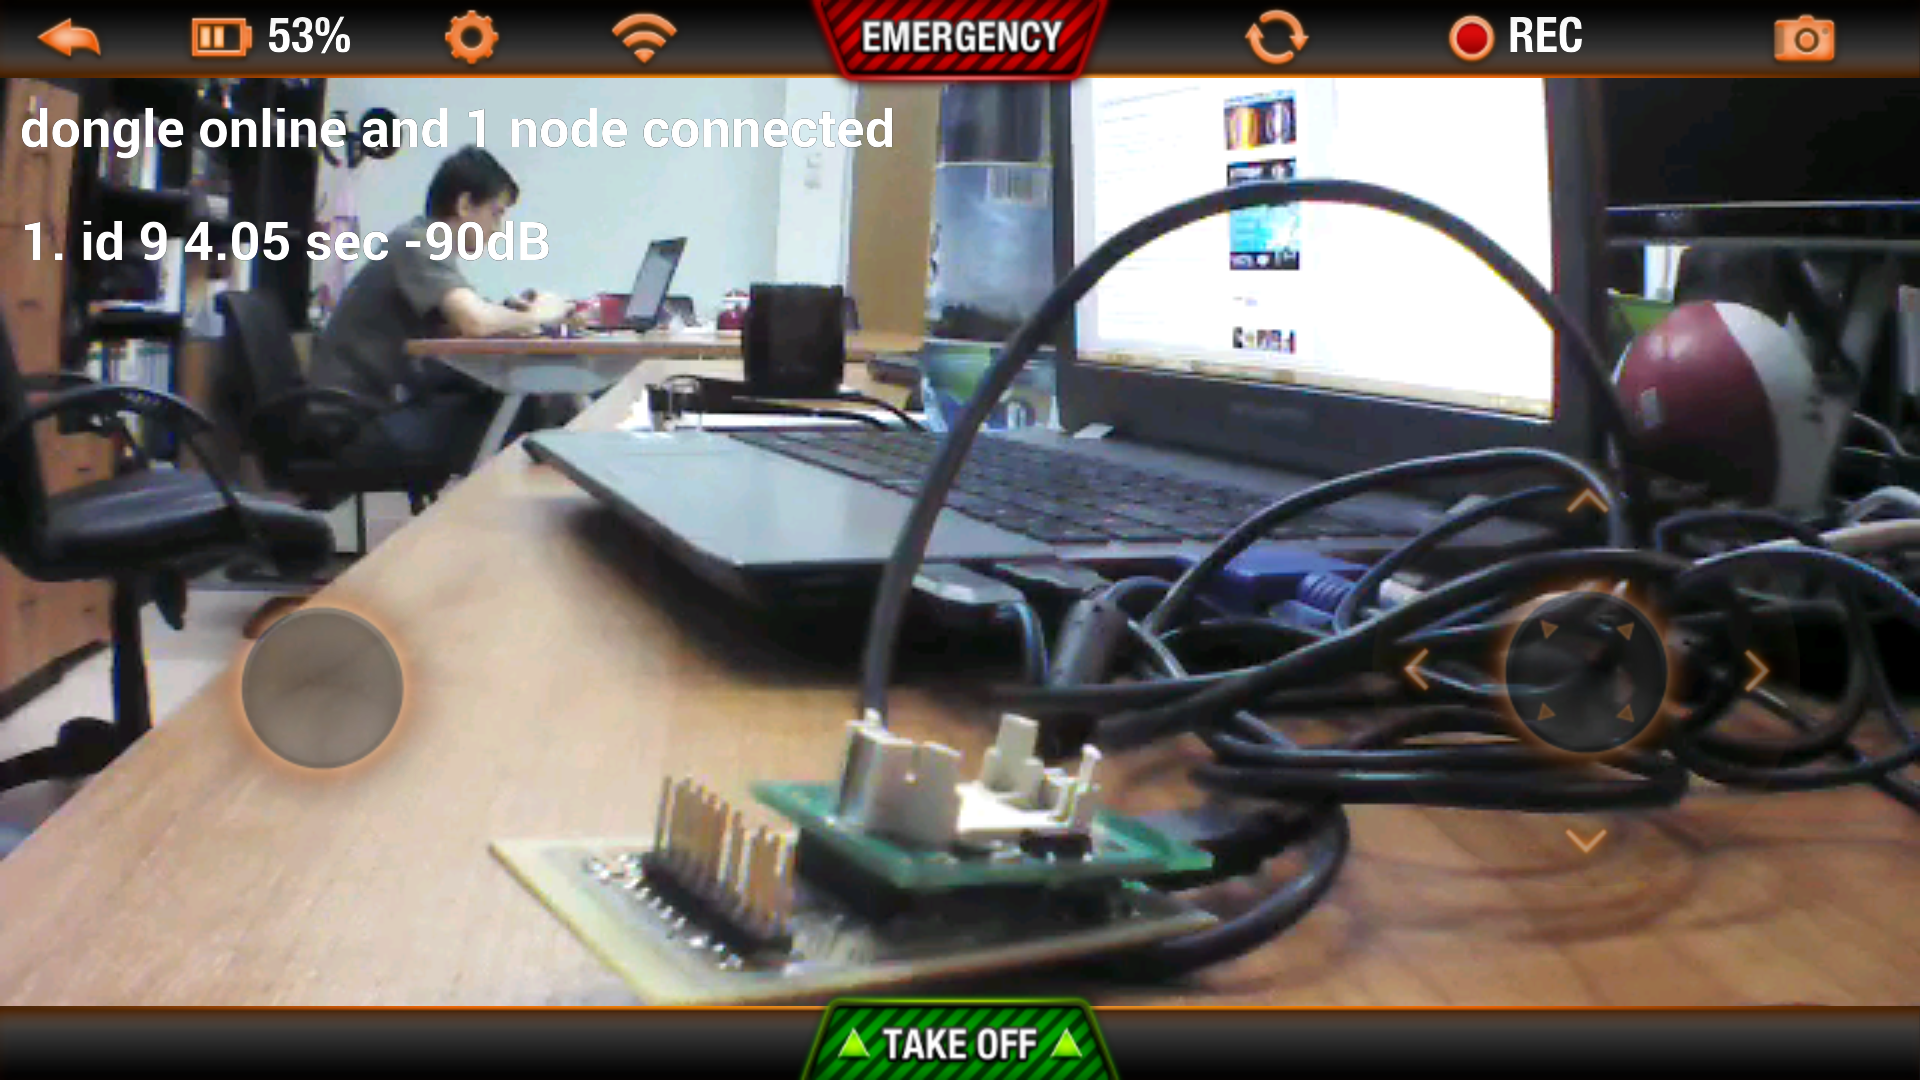
\includegraphics[width=0.9\textwidth]{implementation/android_info.png}
\end{center}
\caption{\small \itshape{ARFreeflight modified Piloting Screen}}
\end{figure}

The Piloting screen of the application has been modified to the display the received data from the drone.

The information displayed consists of the dongle being functional and at most, 9 nodes sorted descending after their signal strength.

\subsection{FTP communication module}

\begin{figure}[ht]
\begin{center}W
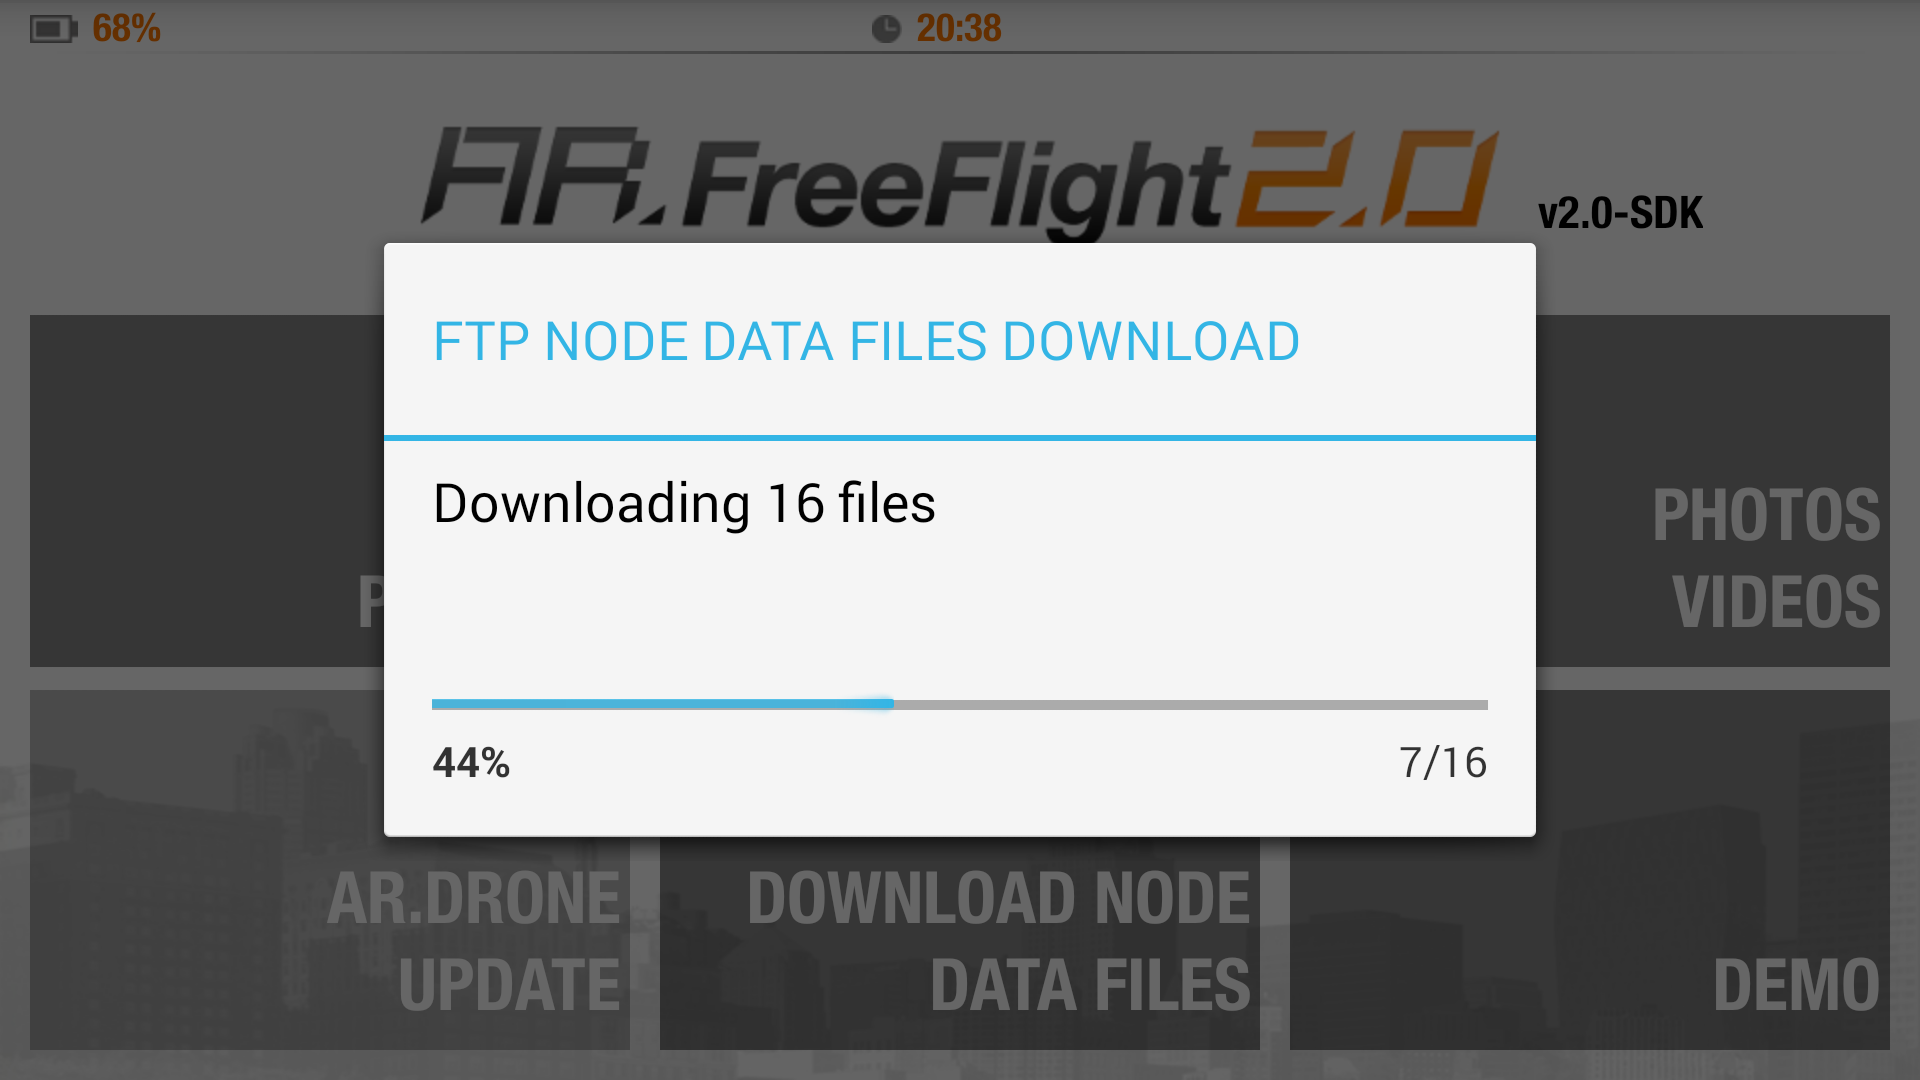
\includegraphics[width=0.9\textwidth]{implementation/android_ftp.png}
\end{center}
\caption{\small \itshape{ARFreeflight FTP downloading files}}
\end{figure}

The drone has a built-in FTP server that can be configured to allow access to any folders/files on the drone. We have configured the drone so that the folder that contains the saved data can be accessed at any time using the 4242 port by any device that has FTP client capabilities. We have added this feature to the Android application as well.

The application will download all the files from the drone to the local storage of the user's Android device while displaying the progress.
